% Constructed and checked from the problem; not a geometric proof.
\documentclass[tikz,border=8pt]{standalone}
\begin{document}
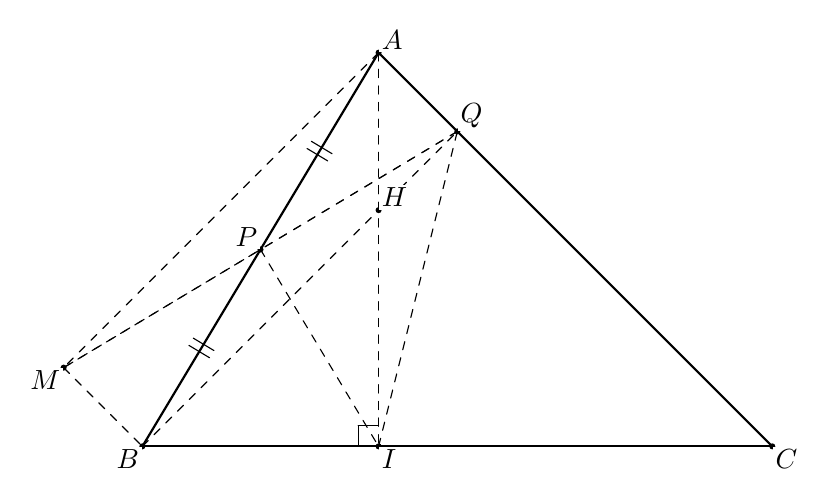
\begin{tikzpicture}[scale=1,line cap=round,line join=round]
\coordinate (p0) at (3,5);
\coordinate (p1) at (0,0);
\coordinate (p2) at (8,0);
\coordinate (p3) at (3,0);
\coordinate (p4) at (-1,1);
\coordinate (p5) at (1.5,2.5);
\coordinate (p6) at (4,4);
\coordinate (p7) at (3,3);
\draw[thick] (p0) -- (p1);
\draw[thick] (p1) -- (p2);
\draw[thick] (p0) -- (p2);
\draw[dashed] (p0) -- (p3);
\draw[dashed] (p0) -- (p4);
\draw[dashed] (p4) -- (p1);
\draw[dashed] (p4) -- (p5);
\draw[dashed] (p6) -- (p4);
\draw[dashed] (p6) -- (p5);
\draw[dashed] (p1) -- (p6);
\draw[dashed] (p6) -- (p0);
\draw[dashed] (p5) -- (p3);
\draw[dashed] (p3) -- (p6);
\draw (3,0.2601) -- (2.7399,0.2601);
\draw (2.7399,0.2601) -- (2.7399,0);
\draw (2.4087477,3.7172009) -- (2.1463548,3.8746366);
\draw (2.3536452,3.6253634) -- (2.0912523,3.7827991);
\draw (0.9087477,1.2172009) -- (0.6463548,1.3746366);
\draw (0.8536452,1.1253634) -- (0.5912523,1.2827991);
\fill (p0) circle (1.1pt) node[fill=white,inner sep=1pt,above right] {$A$};
\fill (p1) circle (1.1pt) node[fill=white,inner sep=1pt,below left] {$B$};
\fill (p2) circle (1.1pt) node[fill=white,inner sep=1pt,below right] {$C$};
\fill (p3) circle (1.1pt) node[fill=white,inner sep=1pt,below right] {$I$};
\fill (p4) circle (1.1pt) node[fill=white,inner sep=1pt,below left] {$M$};
\fill (p5) circle (1.1pt) node[fill=white,inner sep=1pt,above left] {$P$};
\fill (p6) circle (1.1pt) node[fill=white,inner sep=1pt,above right] {$Q$};
\fill (p7) circle (1.1pt) node[fill=white,inner sep=1pt,above right] {$H$};
\end{tikzpicture}
\end{document}
